\chapter{Matematické intermezzo: komplexné čísla}
\label{mat.komplex}

Vieš, že odmocnina z $x$ (označovaná $\sqrt{x}$) je také číslo $y$, že $y^2=x$. 
Majú všetky čísla odmocninu? Ako sa to vezme. Takú $\sqrt{2}$
starí Gréci za číslo nepovažovali: vedeli totiž, že $\sqrt{2}$ sa nedá vyjadriť ako\indexItem{Mat}{ odmocnia z $2$ nie je racionálne číslo}
žiaden zlomok. Ako to mohli vedieť? No nech by $\sqrt{2}=p/q$. Keby $p$ aj 
$q$ bolo párne, tak môžeme obidve vydeliť dvomi a rovnosť stále platí, takže keby
sa $\sqrt{2}$ dala zapísať zlomkom, dá sa zapísať aj takým, že najviac jedno z čísel
$p$, $q$ je párne. Keď si rovnosť vynásobíme samu sebou, máme 
$2=p/q\cdot p/q=p^2/q^2$ a preto $p^2=2q^2$.
Keďže $p^2$ je párne, aj $p$ musí byť párne\footnote{%
Lebo súčin dvoch nepárnych čísel je vždy nepárny. Tu má zmysel nakresliť obrázok, ktorý
budeme za chvíľu aj tak potrebovať:

  \centerline{\tikz[xscale=0.45,yscale=0.6]{
    \filldraw[fill=green!10!white](0,0) rectangle (3,1);
    \filldraw[fill=yellow!10!white](3,0) rectangle (5,1);
    \filldraw[fill=orange!10!white](0,1) rectangle (3,2);
    \filldraw[fill=cyan!10!white](3,1) rectangle (5,2);

    \node[rotate=90,anchor=south] at(0,0.5){$a$};
    \node[rotate=90,anchor=south] at(0,1.5){$b$};
    \node[anchor=south] at(1.5,2){$x$};
    \node[anchor=south] at(3.5,2){$y$};

  }}
Obdĺžnik na obrázku má obsah $(a+b)(x+y)$ a skladá sa zo štyroch menších obdĺžnikov,
preto $(a+b)(x+y)=ax+ay+bx+by$. Keď násobím dve nepárne čísla, mám 
$(2r+1)(2s+1)=4rs+2r+2s+1$, čo je nepárne.
}. Keďže $p$ je párne, $p^2$ je deliteľné $4$. Ale $q$ je nepárne, preto aj $q^2$ je nepárne,
a preto $2q^2$ nie je deliteľné 4. 


Medzičasom sa $\sqrt{2}$ dostala medzi čísla (hovorí sa, že je {\em iracionálne číslo});
za číslo sa dnes považuje kde-čo (napr. si videl takú divočinu ako $\pi$). Môžeme
teda povedať, že všetky kladné čísla majú odmocniny. Ale čo záporné? Tie ich mať
nemôžu, lebo či už je $y$ kladné alebo záporné, $y^2$ je kladné vždy. Takže žiadne
$y$ nemôže byť, trebárs, $\sqrt{-1}$. Ale v matematike máme výhodu: ak niečo neexistuje,
môžeme si to vymyslieť. Takže si môžeme predstaviť, že nejakým spôsobom $\sqrt{-1}$ existuje.
Nebude to žiadne číslo, ako ich doteraz poznáme (hovoríme im {\em reálne}), ale bude to 
{\em niečo}. Nazvem si ho $i$. Chcem, aby sa $i$ pri násobení a sčítaní
správalo, ako sa na čísla patrí,
takže napr. $i+2=2+i$, $i+i+i=3i$, $3(i+7)=3i+21$ a pod. so všetkým. 
Keď mám výraz zložený zo sčítania, násobenia a zátvoriek, vždy ho viem upraviť na
tvar $x+yi$ pre nejaké $x$, $y$. To je preto, že $i^2=-1$, napr.
$(3i+4-i)(i+i-6)+7i-8=(2i+4)(2i-6)+7i-8=4i^2-12i+8i-24+7i-8=3i-28$.
Zjednodušovanie, samozrejme, platí aj ďalej, $i^3=i^2i=-i$, $i^4=i^2i^2=-1\cdot-1=1$, a 
tak ďalej.

 Reálne čísla si zvykneme kresliť na číselnú os. Kam ale nakresliť $i$? na číselnej osi 
už nie je miesto. Poďme preto do roviny: číslo $x+yi$ si nakreslím do bodu so 
súradnicami $[x,y]$, takže napr. $i$ bude nakreslené v bode $[0,1]$.
Keď si rovnako dobre predstavím číslo $x+yi$ ako šípku, ktorá ide z bodu 
$[0,0]$ do bodu $[x,y]$, tak sčítanie funguje veľmi prirodzene: zoberiem jedno
číslo (šípku) a priložím ho na koniec druhého. Napr. 
$(15+4i)+(3+8i)=18+12i$ vidno takto: 


\centerline{
\begin{tikzpicture}[scale=0.27]
  \tikzstyle{vecs}= [-{>[length=2ex,width=1.7ex]}]
  \def\dot(#1,#2){\fill (#1,#2)circle (3.5pt) }
  \draw[dotted,thin,gray] (-3,-2) grid (22,12);
  \draw[red,style=vecs](0,0) -- (15,4);
  \draw[blue,style=vecs](0,0) -- (3,8);
  \draw[blue,style=vecs](15,4) -- (18,12);
  \draw[dashed](3,8)--(18,12);
  \draw[magenta,style=vecs](0,0)--(18,12);
  \dot(0,0) node[anchor=north west]{$[0,0]$};
  \dot(15,4) node[anchor=north west]{$[15,4]$};
  \dot(3,8) node[anchor=south east]{$[3,8]$};
  \dot(18,12) node[anchor=south west]{$[18,12]$};
  \draw[thin] (-3.5,0) -- (22.5,0) (0,-2.5) -- (0,12.5);
\end{tikzpicture}}


Ako si ale predstaviť násobenie? Napr. 
$(1+2i)(3+i)=3+i+6i+2i^2=1+7i$. 
Lepšie to vidno v tzv. {\em polárnych súradniciach}.
Keď chceme jednoznačne určiť bod v rovine, namiesto $x$-ovej a $y$-ovej súradnice
nám stačí pamätať si, pod akým uhlom a ako ďaleko treba ísť.
V kapitole~\ref{sect:editor} sme hovorili o funkciách $\sin$ a $\cos$, takže vieš, že
bod, do ktorého sa ide pod uhlom $\alpha$ do vzdialenosti $r$ má súradnice
$[r\cos\alpha,r\sin\alpha]$, a teda reprezentuje číslo $r\cos\alpha+ir\sin\alpha$.


\centerline{
  \begin{tikzpicture}[scale=4]
  \def\an{40}
  \def\ra{0.4ex}
    \draw[thin,dotted,step=0.5](-0.5,-0.5) grid (1,1);
    \draw(1.1,0) -- (0,0) node[anchor=north east]{$[0,0]$} -- (\an:1.1);

    \draw[red](1ex,0) arc (0:\an:1ex) node[midway,anchor=west]{$\alpha$};
    \draw[thin,gray](-35:1) arc (-35:125:1);

    \draw[-{>[length=3ex,width=1ex]},thin,gray] (0,0) -- (110:1) node[midway,anchor=east]
    {$r$};

    \coordinate (B) at (\an:1);
    \draw[red](0,0)--(B) node[midway,anchor=south east]{$r$};
    %\node[anchor = south east] at (B)  {$[r\cos\alpha,r\sin\alpha]$};

    \coordinate (A) at (B|-0,0) ;
    \draw (B) -- (A) node[midway,anchor=north,rotate=90]{$r\sin\alpha$};
    \draw[draw=none](0,0)--(A)  node[midway,anchor=north]{$r\cos\alpha$};
    \filldraw (B) circle (.2pt);
    
    \draw (A)+(0,\ra) arc (90:180:\ra);
    \filldraw (A)+(-\ra/3,\ra/3) circle (.1pt);

    \def\g{rgb:green,5;yellow,4;blue,2;black,3}
\end{tikzpicture}}

Zoberme si teraz súčin dvoch čísel 
$(r_1\cos\alpha_1+ir_1\sin\alpha_1)(r_2\cos\alpha_2+ir_2\sin\alpha_2)$. Po zjednodušení
z toho dostaneme
\begin{equation}
  \label{eqn:nasobkomplex}
  r_1r_2(\cos\alpha_1\cos\alpha_2-\sin\alpha_1\sin\alpha_2)+
ir_1r_2(\sin\alpha_1\cos\alpha_2+\cos\alpha_1\sin\alpha_2)
.\end{equation}
Môžme to ďalej nejak zjednodušiť? 
Začneme s pravouhlým $\triangle ABC$ s uhlom $\beta$. 
Ak $|AC|=1$, tak $|AB|=\cos\beta$ a $|BC|=\sin\beta$.
Pod úsečkou $AB$ zostrojíme pravouhlý $\triangle ABD$ s uhlom $\alpha$, 
takže $|BD|=\cos\beta\sin\alpha$, $|AD|=\cos\beta\cos\alpha$.
Nakoniec dorobíme ohraničujúci obdĺžnik $ADXY$.



\centerline{\begin{tikzpicture}[scale=8]
  \def\ra{0.4ex}
  \def\bt{35}
  \def\al{30}
  \pgfmathsetmacro{\alc}{180+90-\al}
  \filldraw[fill=red!10!white] (0,0) node[anchor=east]{$A$} 
   -- (\bt:1) node[midway, rotate=\bt, anchor=south ]{1}  
   node[anchor=south west]{$C$} coordinate (C) 
   -- (C|-0,0) node[midway,anchor=south, rotate=90]{{\small$\sin\beta$}} 
   node[anchor=north west]{$B$} coordinate (B) 
   -- (0,0) node[midway,anchor=south]{{\small$\cos\beta$}};
  \draw(0.7ex,0) arc (0:\bt:0.7ex) node[midway,anchor=west]{$\beta$}; 
    \draw (B)+(0,\ra) arc (90:180:\ra);
    \filldraw (B)+(-\ra/3,\ra/3) circle (.1pt);
  \coordinate (D) at (intersection cs: first line = {(0,0) -- (-\al:1)} ,
  second line = {(B) -- ($ (B) + (\alc:1) $)}
  );
  \filldraw[fill=green!10!white](0,0) -- (B) -- 
  (D) node[midway,anchor=north,rotate=90-\al] {{\small$\cos\beta\sin\alpha$}}
  node[anchor=north]{$D$}-- (0,0)
  node[midway,anchor=north,rotate=0-\al] {{\small$\cos\beta\cos\alpha$}}
  ; 
  \draw(1ex,0) arc (0:-\al:1ex) node[midway,anchor=west]{$\alpha$};
  \pgfmathsetmacro{\tmp}{180-\al}
    \draw ($(D)!\ra!(0,0)$) arc (\tmp:\tmp-90:\ra);
    \filldraw (D)+(-0.1*\ra,\ra/2.5) circle (.1pt);

  \coordinate (X) at (intersection cs:   
  first line={ (D) -- ($(D)!3!(B)$)},
  second line={(C) -- ($(C)+(D)$)}) ;

  \coordinate (Y) at ($(X)+([scale=-1]D)$);

  \node[anchor=west] at (X) {$X$};
  \node[anchor=south] at (Y) {$Y$};

  \draw (B) -- (X) -- (Y) -- (0,0);

  \draw[blue] 
  ($(0,0)!0.5ex!(D)$) arc (-\al:\bt:0.5ex)
  ($(0,0)!0.54ex!(D)$) arc (-\al:\bt:0.54ex)
  ($(C)!0.5ex!(Y)$) arc (180-\al:180+\bt:0.5ex)
  ($(C)!0.54ex!(Y)$) arc (180-\al:180+\bt:0.54ex)
  node[midway,anchor=east]{$\alpha+\beta$}
  ;

  \draw[red]($(B)!0.8ex!(X)$) arc (90-\al:90:0.8ex)
  node[midway,anchor=south]{$\alpha$}
  ;

  \draw[draw=none](B) -- (X) node[midway,red,rotate=90-\al,anchor=north]
  {{\small$\sin\beta\cos\alpha$}};
  \draw[draw=none](X) -- (C) node[midway,red,rotate=0-\al,anchor=south]
  {{\small$\sin\beta\sin\alpha$}};

  \draw[draw=none](Y)--(C) node[midway,blue,rotate=0-\al,anchor=south]
  {{\small$\cos(\alpha+\beta)$}};
  \draw[draw=none](0,0)--(Y) node[midway,blue,rotate=90-\al,anchor=south]
  {{\small$\sin(\alpha+\beta)$}};

\end{tikzpicture}}

Vidno, že $|\angle DBA|=90^\circ-\alpha$, preto $|\angle XBC|=\alpha$.
Pretože $AD\parallel XY$, je $|\angle CAD|=|\angle ACY|=\alpha+\beta$.
Z pravouhlého trojuholníka $\triangle BXC$ doplníme, že $|BX|=\sin\beta\cos\alpha$
a $|XC|=\sin\beta\sin\alpha$. Podobne z pravouhlého $\triangle CYA$ doplníme,
že $|CY|=\cos(\alpha+\beta)$ a $|AY|=\sin(\alpha+\beta)$.
Keď si teraz porovnáme, čo máme napísane na stranách obdĺžnika, zistíme, že
$$\sin(\alpha+\beta)=\cos\beta\sin\alpha+\sin\beta\cos\alpha$$
a
$$\cos(\alpha+\beta)=\cos\beta\cos\alpha-\sin\beta\sin\alpha$$
Keď si to porovnáš s (\ref{eqn:nasobkomplex}), zistíš, že 
$$(r_1\cos\alpha_1+ir_1\sin\alpha_1)(r_2\cos\alpha_2+ir_2\sin\alpha_2)
=r_1r_1\cos(\alpha_1+\alpha_2)+ir_1r_2\sin(\alpha_1+\alpha_2)$$
Inými slovami, ak vynásobím dve komplexné čísla, dostanem číslo, ktorého uhol
v polárnych súradniciach je súčtom uhlov a dĺžka je súčinom dĺžok.
V kartézskych súradniciach by sme napísali 
$(a+bi)(x+yi)=(ax-by)+(bx+ay)i$, špeciálne $(a+bi)^2=(a^2-b^2)+2abi$.


\centerline{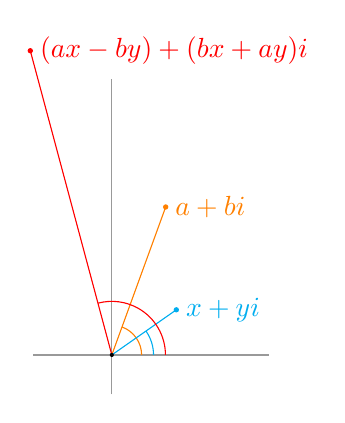
\begin{tikzpicture}[scale=0.5]
  \def\r{4}
  \def\al{70}
  \def\rr{2}
  \def\bt{35}
  \pgfmathsetmacro{\rrr}{\r*\rr}
  \pgfmathsetmacro{\gm}{\al+\bt}
  \def\papek(#1,#2)[#3]#4{%
    \draw[#3] (0,0) -- (#1:#2) [fill=#3] circle (1.5pt);
    \draw[#3] (#4,0) arc (0:#1:#4);
  }
  \draw[gray!80!white,thin] (-2,0) -- (4,0) (0,-1) -- (0,7);
  \papek(\al,\r)[orange]{5ex}
  \papek(\bt,\rr)[cyan]{7ex}
  \papek(\gm,\rrr)[red]{9ex}
 
  \node[orange,anchor=west]at (\al:\r) {$a+bi$};
  \node[cyan,anchor=west]at (\bt:\rr) {$x+yi$};
  \node[red,anchor=west]at (\gm:\rrr) {$(ax-by)+(bx+ay)i$};
  \fill (0,0) circle (1.5pt);

\end{tikzpicture}}

\section*{Projekt: Mandelbrotova množina}
\label{projekt.mandelbrot}

Matematik menom Benoit Mandelbrot sa hral takúto hru\footnote{%
V skutočnosti sa tú hru ako prví hrali Robert Brooks a Peter Matelski v r. 1978,
ale Mandelbrotovi sa tak veľmi páčila, že je pomenovaná po ňom.
}: zobral si nejaké komplexné číslo \indexItem{Mat}{Mandelbrotova množina}
$c$ a začal počítať postupne $c, c^2+c, (c^2+c)^2+c, 
\left((c^2+c)^2+c\right)^2+c,\ldots$ a tak ďalej; vždy ďalšie (komplexné) číslo
získal tak, že to doterajšie umocnil na druhú a prirátal $c$. Niektoré čísla
stále poskakovali okolo toho istého miesta, 
iné začali rásť a rástli donekonečna:


\centerline{
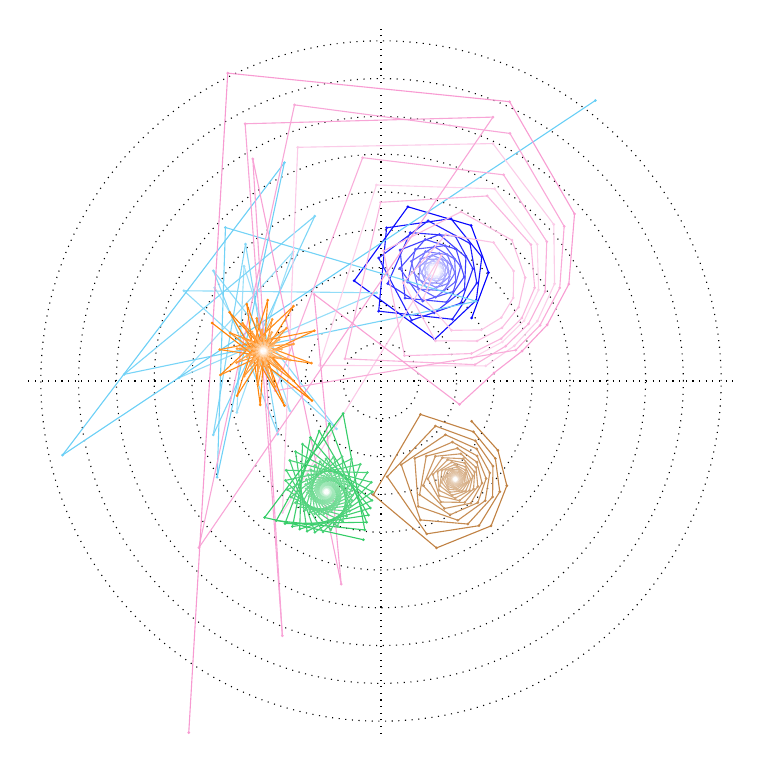
\begin{tikzpicture}[scale=3.2]
  \def\dot(#1,#2){\fill[fill=\clr!\clrval!\clrt] (#1,#2) circle (0.17pt);}

  \def\iter#1{%
    \pgfmathsetmacro{\clrval}{100/\niter*#1}
    \dot(\zx,\zy)
    \pgfmathparse{#1}
    \ifnum\pgfmathresult=0\relax\else
      \pgfmathsetmacro{\nzx}{(\zx*\zx)-(\zy*\zy)+\cx}
      \pgfmathsetmacro{\nzy}{2*\zx*\zy+\cy}
      \draw[\clr!\clrval!\clrt](\zx,\zy) -- (\nzx,\nzy);
      \pgfmathsetmacro\zx{\nzx}
      \pgfmathsetmacro\zy{\nzy}
      \pgfmathtruncatemacro{\n}{#1-1}
      \iter{\n}
    \fi
   }

 
  \def\rng{1.4}
  \draw[thin,dotted] (-\rng,0) -- (\rng,0) (0,-\rng) -- (0,\rng);
  \foreach \r in {0.15,0.3,...,\rng}{
    \draw[thin,dotted] (0,0) circle(\r);
  }



   \foreach \x/\y/\clr/\clrt/\niter in {0.36/0.25/blue/white/100
   ,0-0.66/0.37/cyan!60!white/cyan!60!white/20
   ,0.36/0.09/magenta!40!white/magenta!40!white/72
   ,0-0.67/0.23/orange/white/100
   ,0-0.07/0-0.63/green!50!gray!80!cyan/white/200
   ,0.36/0-0.16/brown/white/200
   } { 
   \pgfmathsetmacro\cx{\x}
   \pgfmathsetmacro\cy{\y}
   \def\zx{\cx}
   \def\zy{\cy}
   %\typeout{start z: \zx, \zy}
   \iter{\niter}
   }
\end{tikzpicture}}

Mandelbrota zaujímalo, ktoré čísla sú také, že nikdy neujdú z kruhu
s polomerom $R$.

\begin{uloha}
  \label{uloha-mandelbrot}
  Na vstupe sú čísla $R$ a $N$. Potom nasledujú komplexné čísla v kartézskych
  súradniciach, t.j. číslo $x+iy$ je zapísané dvojicou \vb{x y}.
  Vstup končí číslo \vb{0 0}. Napíš program, ktorý pre každé číslo
  vypíše \vb{ujde} alebo \vb{neujde}. Číslo ujde, ak počas prvých $N$ 
  Mandelbrotových iterácií jeho veľkosť (t.j. $\sqrt{x^2+y^2}$) prekročí $R$.
  Napr. 


  \begin{column}{0.45}
\begin{outputBox}
100000 100000
0.36 0.25
-0.66 0.37
0.36 0.09
-0.67 0.23
-0.07 -0.63
0.36 -0.16
0 0
\end{outputBox}
\end{column}\hfill
\begin{column}{0.45}
\begin{outputBox}
neujde
ujde
ujde
neujde
neujde
neujde
\end{outputBox}
\end{column}
\end{uloha}

Mandelbrot sa ďalej rozhodol, že si skúsi množinu nakresliť: čierne body budú čísla, 
ktoré neujdú a biele čísla, ktoré ujdú.

\begin{uloha}
  Na vstupe sú čísla $R$, $N$ ako z minulej úlohy. Navyše čísla $d$, $x$, $y$, $m$.
  Napíš program, ktorý vyrobí obrázok rozmerov $n\times n$ zachytávajúci výsek
  komplexnej roviny so stredom $x+iy$ a dĺžkou strany $m$.
  Napr. pre $x=-0.65$, $y=0$, $m=0.3$ by si mal dostať obrázok

  
  {
  \setlength{\fboxsep}{0pt}
  \centerline{\fbox{
\includegraphics[width=0.5\textwidth]{data/82.png}}}
}
\end{uloha}



Čiernym bodom, ktoré si dostal na obrázku, sa hovorí Mandelbrotova množina a má rôzne\indexItem{Mat}{fraktál}
vlastnosti, ktoré sa matematikom páčia: napr. je súvislá a je to {\em fraktál}, t.j.
ak sa pozrieš s väčším priblížením, nájdeš v nej zmenšené kópie celej množiny, aj 
so zmenšenými kópiami \ldots.


Možno si si ale pri hraní sa s parametrami $R$ a $N$ všimol, že pre veľké počty
iterácií program začína bežať dosť dlho. Na zrýchlenie programov je spravidla najúčinnejšie
vymyslieť rýchlejší algoritmus, ale ak to nejde, dá sa povedať kompilátoru, aby sa viac snažil.\indexItem{Prg}{optimalizácia \vb{-O}}
Aj \vb{g++} aj \vb{clang++}  majú 
prepínač \vb{-O} (ako optimalizácia). 
Ak teda pri kompilovaní namiesto \vb{g++ program.cc -o program}
napíšeš \vb{g++ -O3 program.cc -o program}, kompilátor bude pracovať dlhšie, lebo sa bude
snažiť prepísať tvoj program tak, aby robil to isté, ale bežal čo najrýchlejšie. 
Kompilátory sú celkom šikovné, takže niekedy
to dokáže spraviť aj $10\times$ rýchlejšie.


A ešte jedna poznámka. V knižnici \prg!#include<complex>! je definovaný typ\indexItem{Prg}{\vb{complex}}
\prg!complex! na príjemnejšiu prácu s komplexnými číslami.
Je to šablóna, ktorá ako parameter dostane typ súradníc, napr. \prg!complex<double>!.
Komplexné čísla môžeš  sčitovať
a násobiť ako normálne čísla, načítavať zo vstupu v tvare napr. \vb{(-0.65,0)}
a pod. Ak máš \prg!complex<double> z!, tak \prg!z.real()! je $x$-ová (reálna) súradnica, 
\prg!z.imag()! je $y$-ová (imaginárna) súradnica, \prg!norm(z)! je $x^2+y^2$,
\prg!abs(z)! je veľkosť (t.j. $\sqrt{x^2+y^2}$) a \prg!arg(z)! je uhol v radiánoch.


Teraz poďme do obrázku pridať trochu farby. Body, ktoré patria do množiny (t.j. sú čierne),
necháme čierne. Biele body sú tie, ktoré ušli cez $R$ po menej ako $N$ iteráciách. Môžeme 
im dať farbu podľa počtu iterácií, kedy prekročili $R$. 
Ako konkrétne priraďovať farbu? Budeme mať pole (vektor) \vb{paleta}
prednastavených farieb a farbu príslušného pixela v obrázku určíme ako 
\prg!paleta[iter % paleta.size()]!
kde \vb{iter} je počet iterácií, kedy veľkosť prekročila $R$. 


Keď dizajnéri navrhujú palety a farebné schémy, často pracujú so zápisom farby pomocou\indexItem{Alg}{hex-reťazec farby}
reťazca (tzv. {\em hex} reťazec). Takisto ho podporujú rôzne ''color-picker'' nástroje.
Skladá sa zo siedmich (RGB) alebo deviatich (RGBA) znakov
\def\tmp#1{\vb{\textcolor{magenta}{#1}}}
\tmp{\#RRGGBB}, pričom každá z dvojíc \tmp{RR}, \tmp{GG}, \tmp{BB}
je číslo od 0 do 255 zapísané v šestnástkovej sústave\footnote{%
  Šestnástková ({\em hexadecimálna}) sústava používa cifry
  \rmfamily{0,1,2,3,4,5,6,7,8,9,a,b,c,d,e,f} (niekedy môžu byť aj veľké písmená).
  Posledná cifra udáva počet jednotiek, predposledná počet šestnástok, predpredposledná
  počet $16\cdot16=256$-tiek atď. Takže napr {\rmfamily 2b} v šestnástkovej sústave je
  $2\cdot16+11=43$.
}.

\begin{uloha}
  Napíš program, ktorý zo vstupu prečíta veľkosť palety, potom príslušný počet
  hex reťazcov farieb, potom parametre $R$, $N$, rozmery obrázka, stred (komplexné
  číslo) a parameter $m$ ako v predchádzajúcich úlohách a vyrobí farebný obrázok.
  Napr. pre tento vstup by obrázok vyzeral takto:

  
\begin{column}{0.45}  
  \begin{Verbatim}
16
#f44336 #e81e63 #9c27b0 #673ab7
#3f51b5 #2196f3 #03a9f4 #00bcd4
#009688 #4caf50 #8bc34a #cddc39
#ffeb3b #ffc107 #ff9800 #ff5722

1000000 100000 
1600 1200 
(-0.65,0) 0.3
  \end{Verbatim}
\end{column}
  \hspace*{-5ex}
\begin{column}{0.45}
\vskip 0pt
  {
  \setlength{\fboxsep}{0pt}
  \fbox{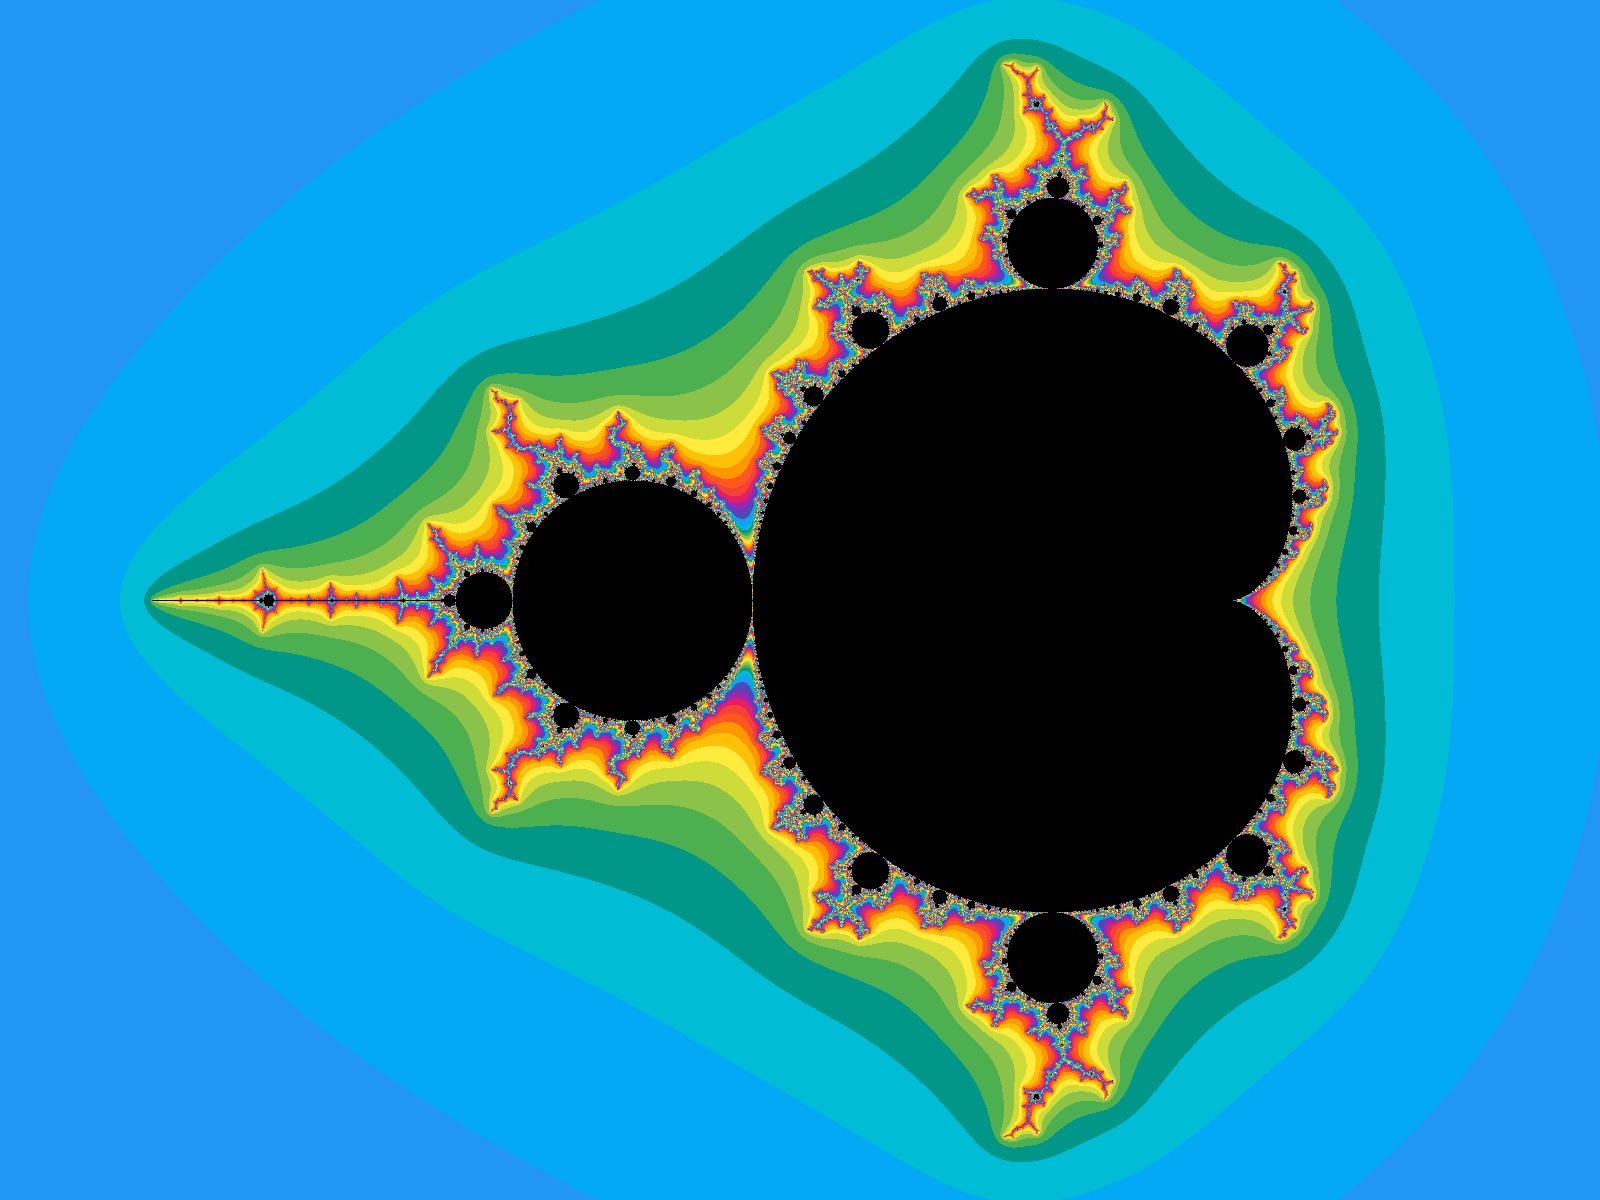
\includegraphics[width=1.3\textwidth]{data/83.png}}
  }\end{column}
\end{uloha}


Pekné, ale stále trochu vadí, že prechody medzi farbami sú náhle. Chcel by som, aby
zafarbenie bolo plynulé. Na to treba vyriešiť dva problémy: ako vyrobiť ''paletu'', v ktorej
sú plynulé prechody a potom ako nahradiť počet iterácií niečím, čo sa plynulejšie mení.


Prvý problém vyriešime pomocou {\em interpolácie} farieb. Interpolácia je vlastne\indexItem{Alg}{interpolácia}
proporcionálne zmie\-ša\-va\-nie: ak mám čísla $a$ a $b$, a parameter $t$, ktorý vyjadruje
časť (t.j. $0\le t\le1$), môžem ich zmiešať tak, že zoberiem $t$-tinu z $a$ a
zvyšok (t.j. $1-t$) doplním z $b$: dostanem $ta+(1-t)b$. Ak je $t=0$, mám $b$, ak je
$t=1$, mám $a$ a ak sa $t$ plynule mení, aj výsledná hodnota plynule prechádza z $b$ do $a$
(pre $t=1/2$ mám priemer). Pre dve farby môžeme urobiť to isté: nezávisle interploáciu
v červenej, zelenej a modrej zložke\footnote{%
Len pre informáciu: existuje veľa rôznych farebných modelov, ktoré tiež reprezentujú farbu
pomocou niekoľkých (spravidla) troch čísel, ale tie čisla nie sú ''červená'', ''zelená'', 
''modrá'',
ale napr. ''farba'',''sýtosť'',''jas'' a pod. Práve RGB model nie je veľmi 
vhodný na interpoláciu po zložkách, na to sú lepšie kolorimetrické modely ako XYZ.
Ale na naše účely to stačí v pohode.
}. Spravme triedu \vb{Gradient}, ktorá bude obsahovať pole zlomových bodov. Zlomový\indexItem{Alg}{farebný gradient}
bod má pozíciu (z rozsahu 0\ldots1) a farbu. \vb{Gradient} potom
pre dané \vb{x} zistí\footnote{%
  napr. binárnym vyhľadávaním, aj keď pre málo zlomových bodov je 
  binárne vyhľadávanie overkill},
  bedzi ktorými zlomovými bodmi sa nachádza, a vráti príslušnú interpoláciu.
  Gradient s troma zlomovými bodmi vyzerá napríklad takto:
  

\centerline{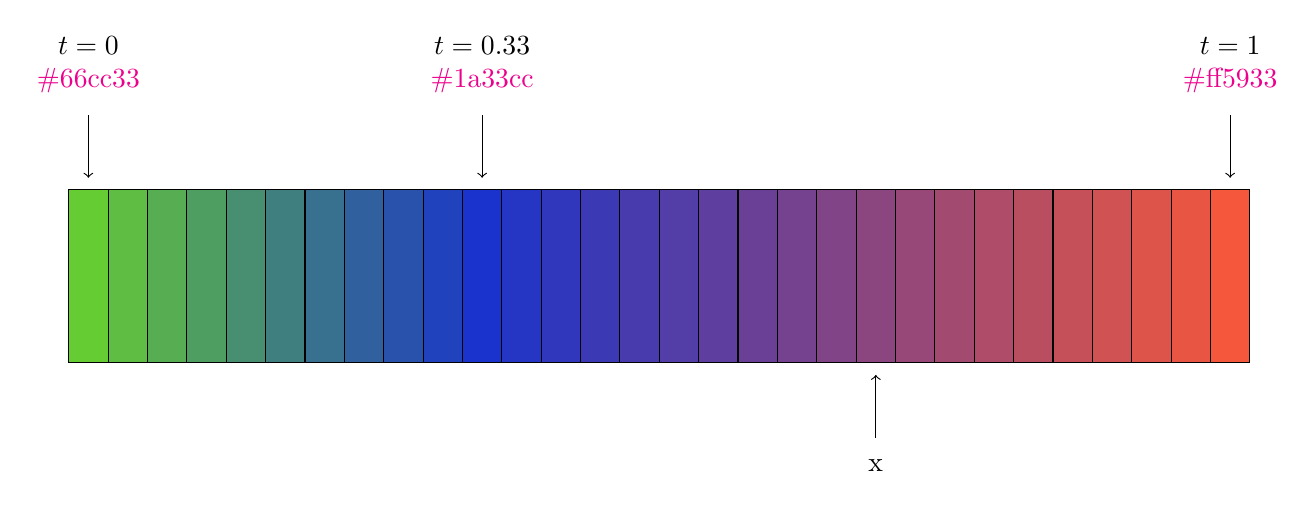
\begin{tikzpicture}[xscale=5,yscale=2.2,
  every text node part/.style={align=center}]
  \def\step{0.1}
  \def\mark(#1)#2#3{%
    \draw[->,shorten <= 1ex , shorten >= 1ex] (#1+0.5*\step,1.5) 
    node[anchor=south]{$t=#2$\\ \textcolor{magenta}{\vb{\##3}}}
    -- (#1+0.5*\step,1);
    }
  \foreach \t in {0,\step,...,1} {
    \pgfmathsetmacro{\r}{0.1*\t+ 0.4*(1-\t)}
    \pgfmathsetmacro{\g}{0.2*\t+ 0.8*(1-\t)}
    \pgfmathsetmacro{\b}{0.8*\t+ 0.2*(1-\t)}
    \definecolor{myfill}{rgb}{\r,\g,\b}
    \filldraw[fill=myfill](\t,0) rectangle (\t+\step,1);
  }
  \begin{scope}[shift={(1,0)}]
  \foreach \t in {0,\step,...,2} {
    \pgfmathsetmacro{\ts}{0.5*\t}
    \pgfmathsetmacro{\r}{1*\ts+ 0.1*(1-\ts)}
    \pgfmathsetmacro{\g}{0.35*\ts+ 0.2*(1-\ts)}
    \pgfmathsetmacro{\b}{0.2*\ts+ 0.8*(1-\ts)}
    \definecolor{myfill}{rgb}{\r,\g,\b}
    \filldraw[fill=myfill](\t,0) rectangle (\t+\step,1);
  }
  \end{scope}
  \mark(0){0}{66cc33}
  \mark(1){0.33}{1a33cc}
  \mark(3-\step){1}{ff5933}

  \draw[->,shorten <= 1ex , shorten >= 1ex] (2+0.5*\step,-0.5)
  node [anchor=north]{\vb{x}}-- (2+0.5*\step,0);
\end{tikzpicture}}


S pomocou knižnice \vb{cmath}, v ktorej je funkcia \vb{fmod}: zvyšok\indexItem{Prg}{\vb{fmod}}
po delení, ale pre desatinné čísla (t.j. \prg!fmod(t,1)! je desatinná
časť z \vb{t}) môže implementácia vyzerať napr. takto:


\begin{lstlisting}
struct Stop {
  double t;
  RGBA f;
};

struct Gradient {
  vector<Stop> stops;

  Gradient(const vector<Stop>& _stops) { stops = _stops; }

  RGBA operator()(double t) {
    t=fmod(t,1);
    RGBA x;
    auto it = lower_bound(stops.begin(), stops.end(), Stop{t, {}},
                          [](Stop a, Stop b) { return a.t < b.t; });

    if (it == stops.begin()) return stops[0].f;
    RGBA a = (it)->f, b = (it - 1)->f;
    t = (t - (it - 1)->t) / (it->t - (it - 1)->t);

    x.r = (Byte)(t * a.r + (1 - t) * b.r);
    x.g = (Byte)(t * a.g + (1 - t) * b.g);
    x.b = (Byte)(t * a.b + (1 - t) * b.b);
    return x;
  }
};
\end{lstlisting}


Druhý problém je, akú hodnotu použiť namiesto počtu iterácií, aby sa menila spojitejšie.
Po troche hrania sa mi osvedčilo toto: pre každý pixel si zapamätám počet iterácií a
jeho veľkosť v čase keď prekročil hranicu (kvôli väčšej plynulosti beriem logaritmus
z veľkosti; v knižnici \vb{cmath} je na to funkcia \vb{log}). Potom, keď som mal
hotový celý obrázok, tak som zistil všetky počty iterácií, ktoré sa vyskytli a pre každý počet iterácií našiel maximálnu a minimálnu hodnotu
veľkosti. Každý pixel potom dostal okrem počtu iterácií aj desatinnú časť, ktorá závisela od
jeho veľkosti (relatívne k maximálnej a minimálnej veľkosti pre tento počet iterácií).


\begin{column}{0.45}
\vskip 0pt
\begin{lstlisting}
Gradient g(
{{0.0, RGBA(0, 7, 100)},
{0.16, RGBA(32, 107, 203)},
{0.42, RGBA(237, 255, 255)},
{0.6425, RGBA(255, 170, 0)},
{0.8575, RGBA(0, 2, 0)},
{1.0, RGBA(0, 7, 100)}});
\end{lstlisting}
\end{column}
\hfill
\begin{column}{0.45}
\vskip 0pt
\centerline{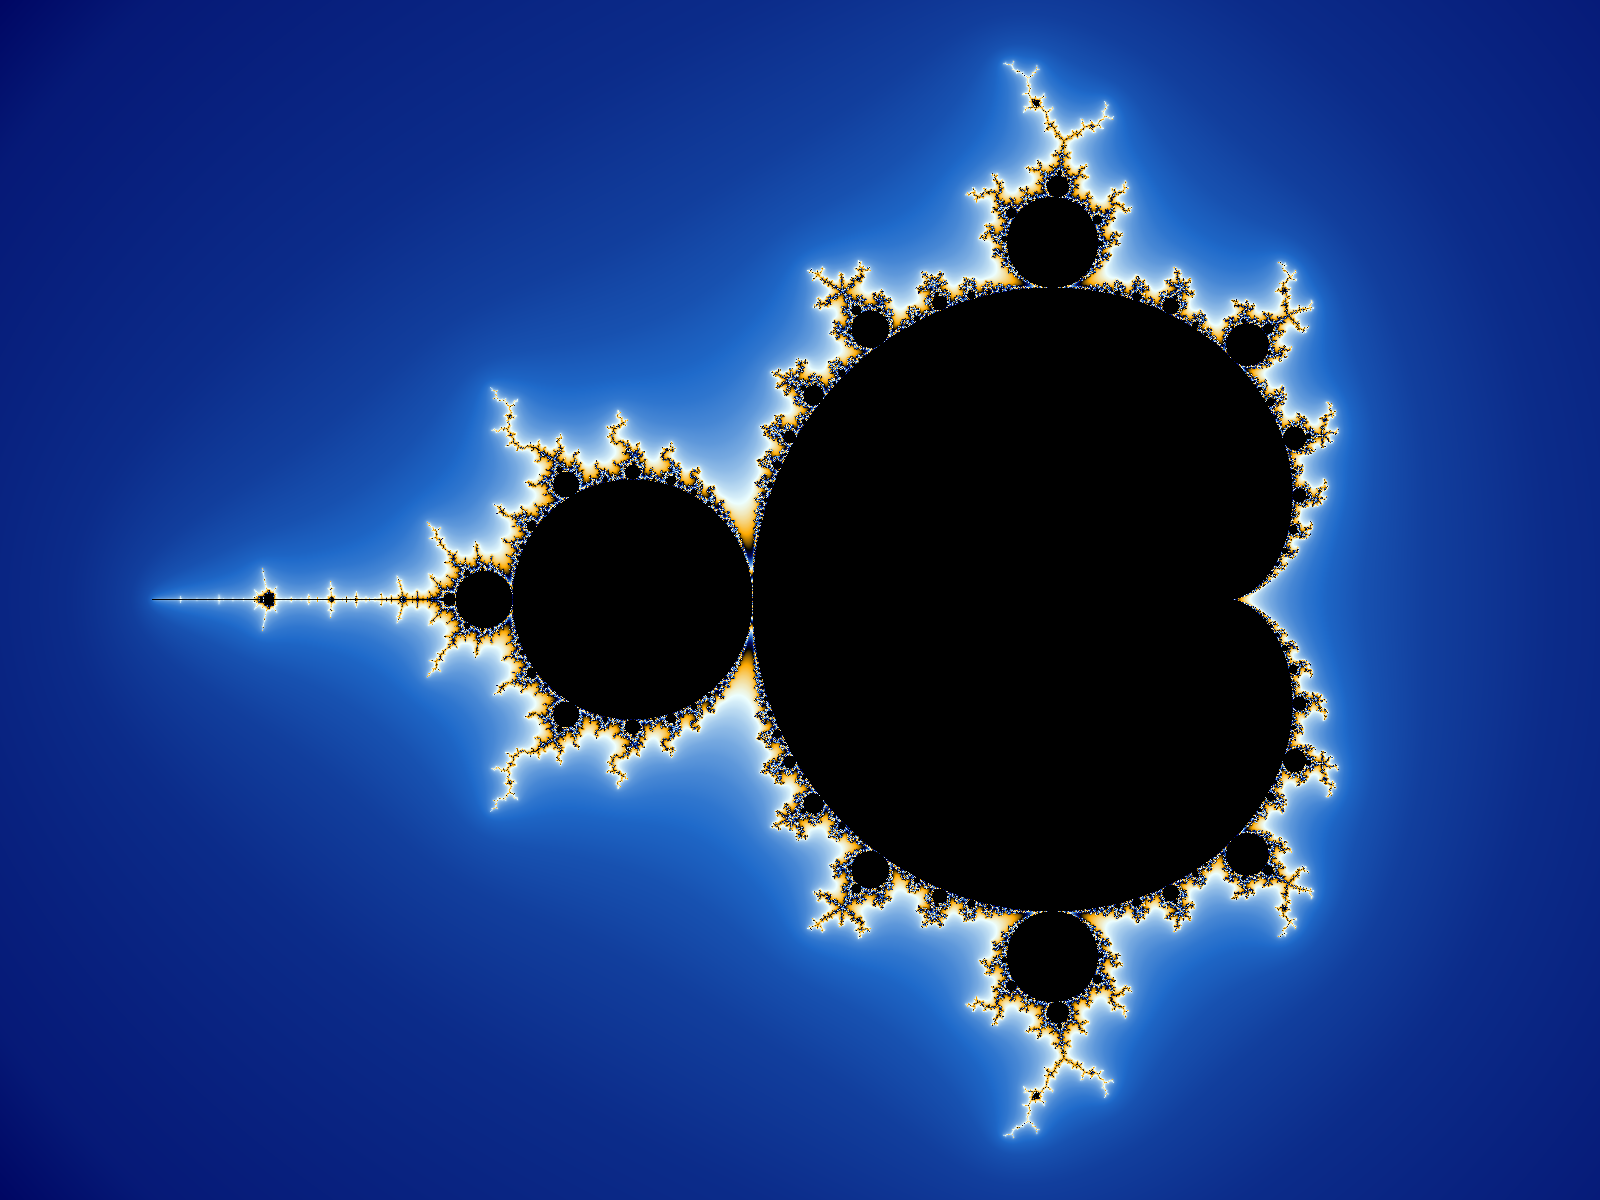
\includegraphics[width=1.1\textwidth]{data/mb.png}}
\end{column}


\begin{column}{0.45}
\vskip 0pt
\centerline{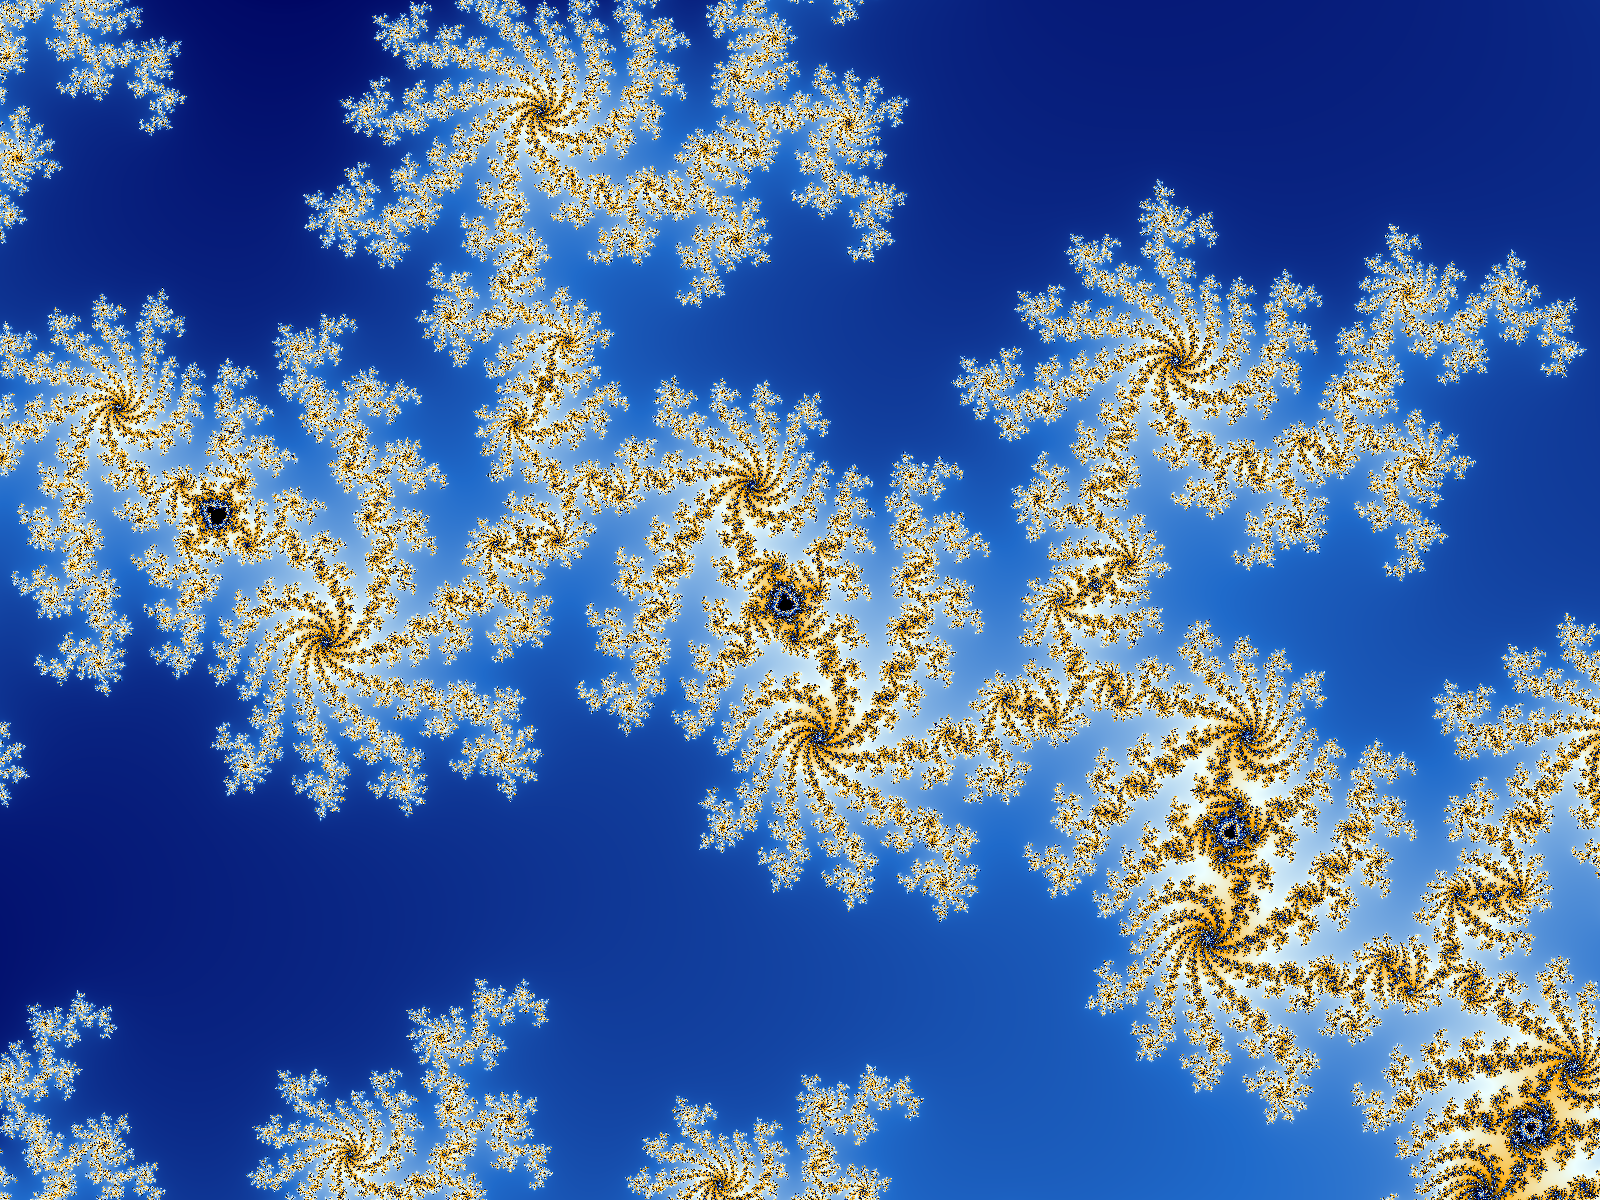
\includegraphics[width=1.1\textwidth]{data/mb1.png}}
\centerline{stred $(-0.6928223,0.3282697)$}
\centerline{$m=508.9334$}
\end{column}
\hfill
\begin{column}{0.45}
\vskip 0pt
\centerline{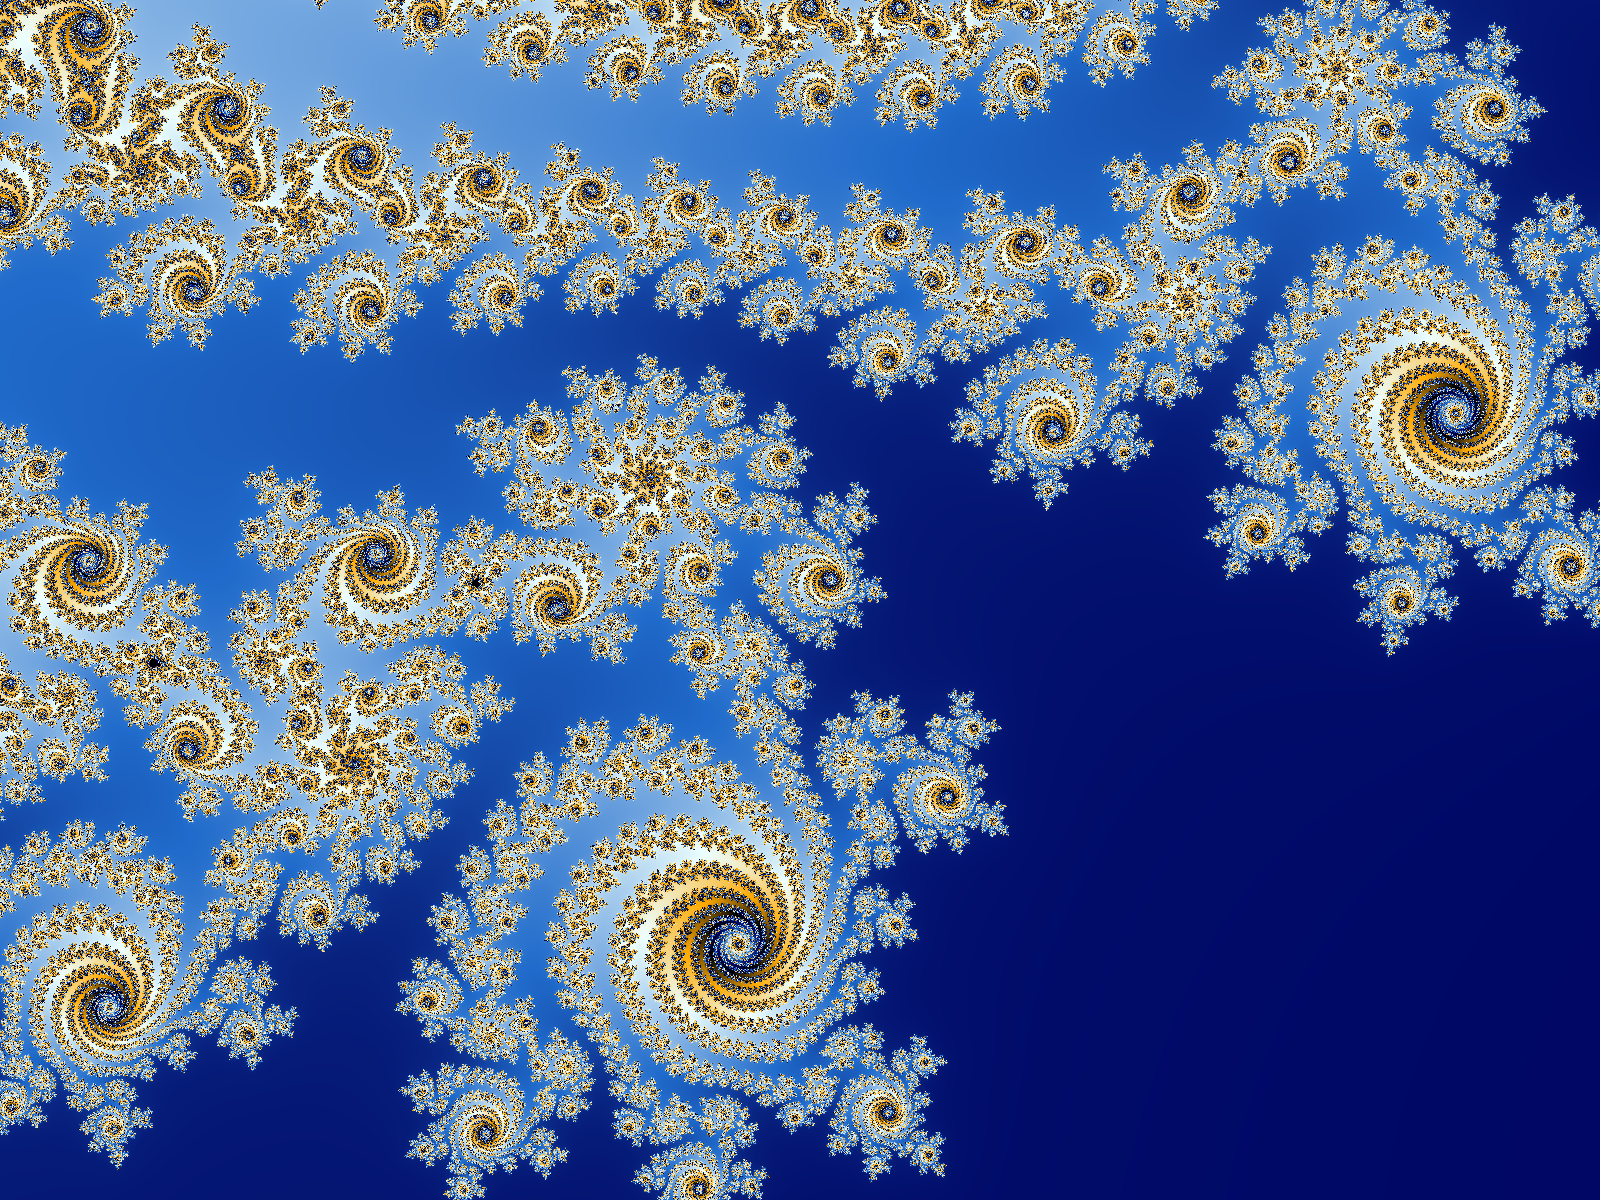
\includegraphics[width=1.1\textwidth]{data/mb2.png}}
\centerline{stred $(-0.59990625,-0.4290703125)$}
\centerline{$m=1500$}
\end{column}


\begin{column}{0.45}
\vskip 0pt
\centerline{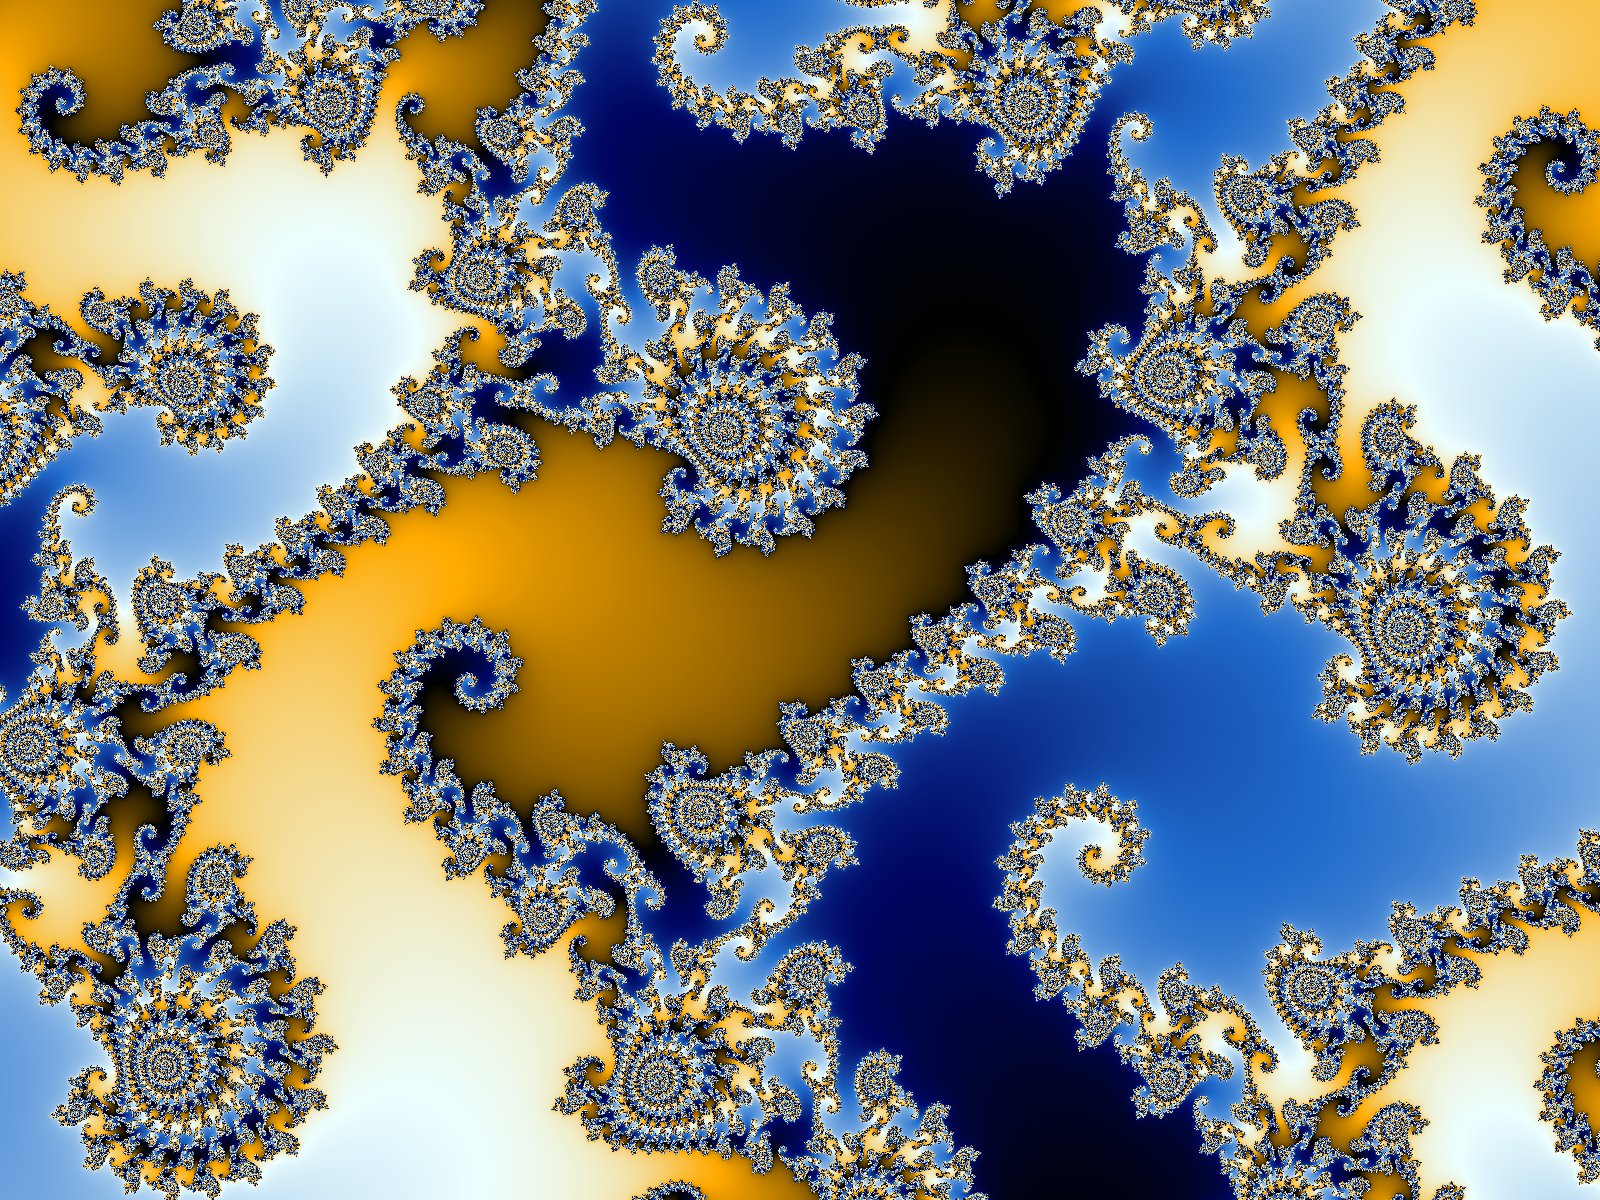
\includegraphics[width=1.1\textwidth]{data/mb3.png}}
\centerline{stred $(-0.743643887035763,0.13182590421259918)$}
\centerline{$m=4.3e14$}
\end{column}
\hfill
\begin{column}{0.45}
\vskip 0pt
\centerline{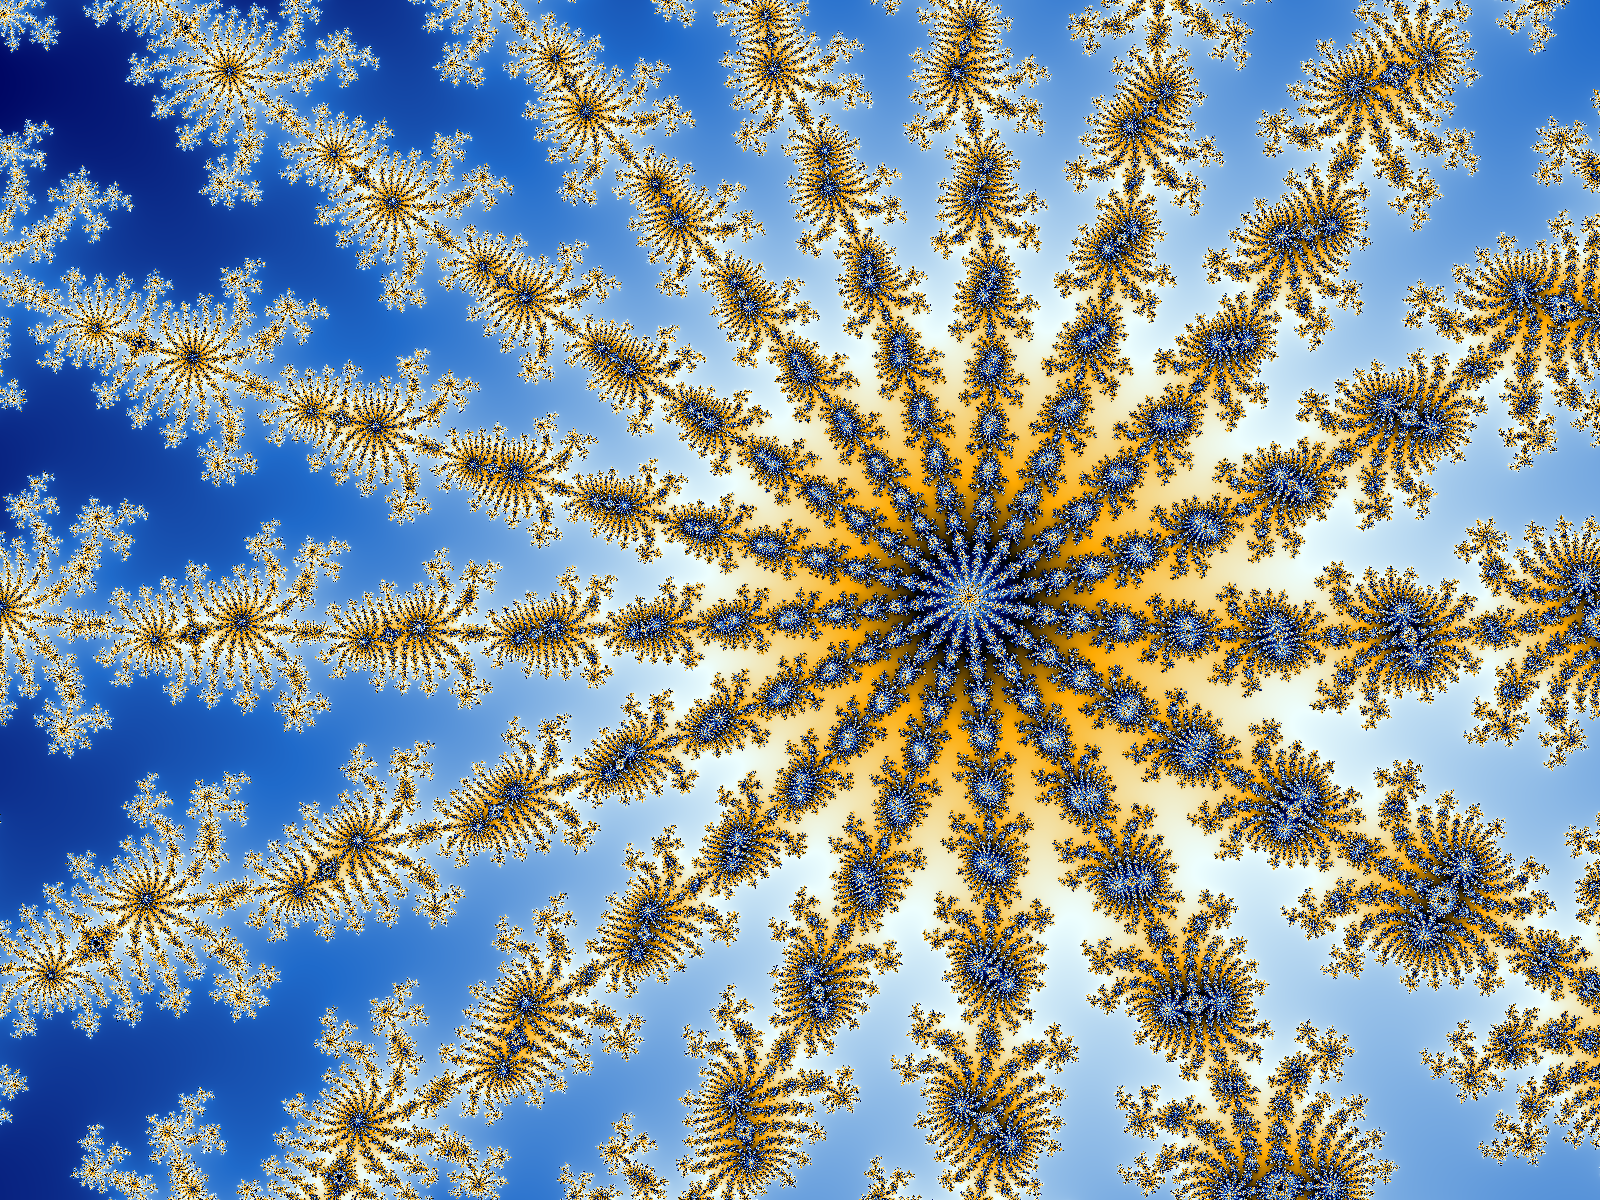
\includegraphics[width=1.1\textwidth]{data/mb4.png}}
\centerline{stred $(-0.65550685,0.3783525)$ }
\centerline{$m=236.2$}
\end{column}

\begin{uloha}
  Pohraj sa s Mandelbrotovou množinou.
\end{uloha}

